%% LyX 2.1.4 created this file.  For more info, see http://www.lyx.org/.
%% Do not edit unless you really know what you are doing.
\documentclass[oneside]{book}
\usepackage[T1]{fontenc}
\usepackage[utf8]{luainputenc}
\setcounter{secnumdepth}{3}
\setcounter{tocdepth}{3}
\usepackage{wrapfig}
\usepackage{graphicx}

\makeatletter
\@ifundefined{date}{}{\date{}}
\makeatother

\begin{document}

\title{Robótica educativa con software y hardware libre en colegios técnicos}

\maketitle

\section*{Fundamentación}

ICARO es un proyecto colaborativo sin fines de lucro, que trata de
acercar de manera sencilla las nociones básicas de la electrónica
y la programación en un entorno robótico para utilizarlo dentro del
aula como una herramienta de aprendizaje. 

La robótica educativa, dado su carácter multidisciplinario, permite
el abordaje de conocimientos variados como la electrónica, informática,
física y matemática mediante la construcción de un juguete-objeto
como puede ser un robot. \begin{wrapfigure}{o}{0.5\columnwidth}%
\begin{centering}
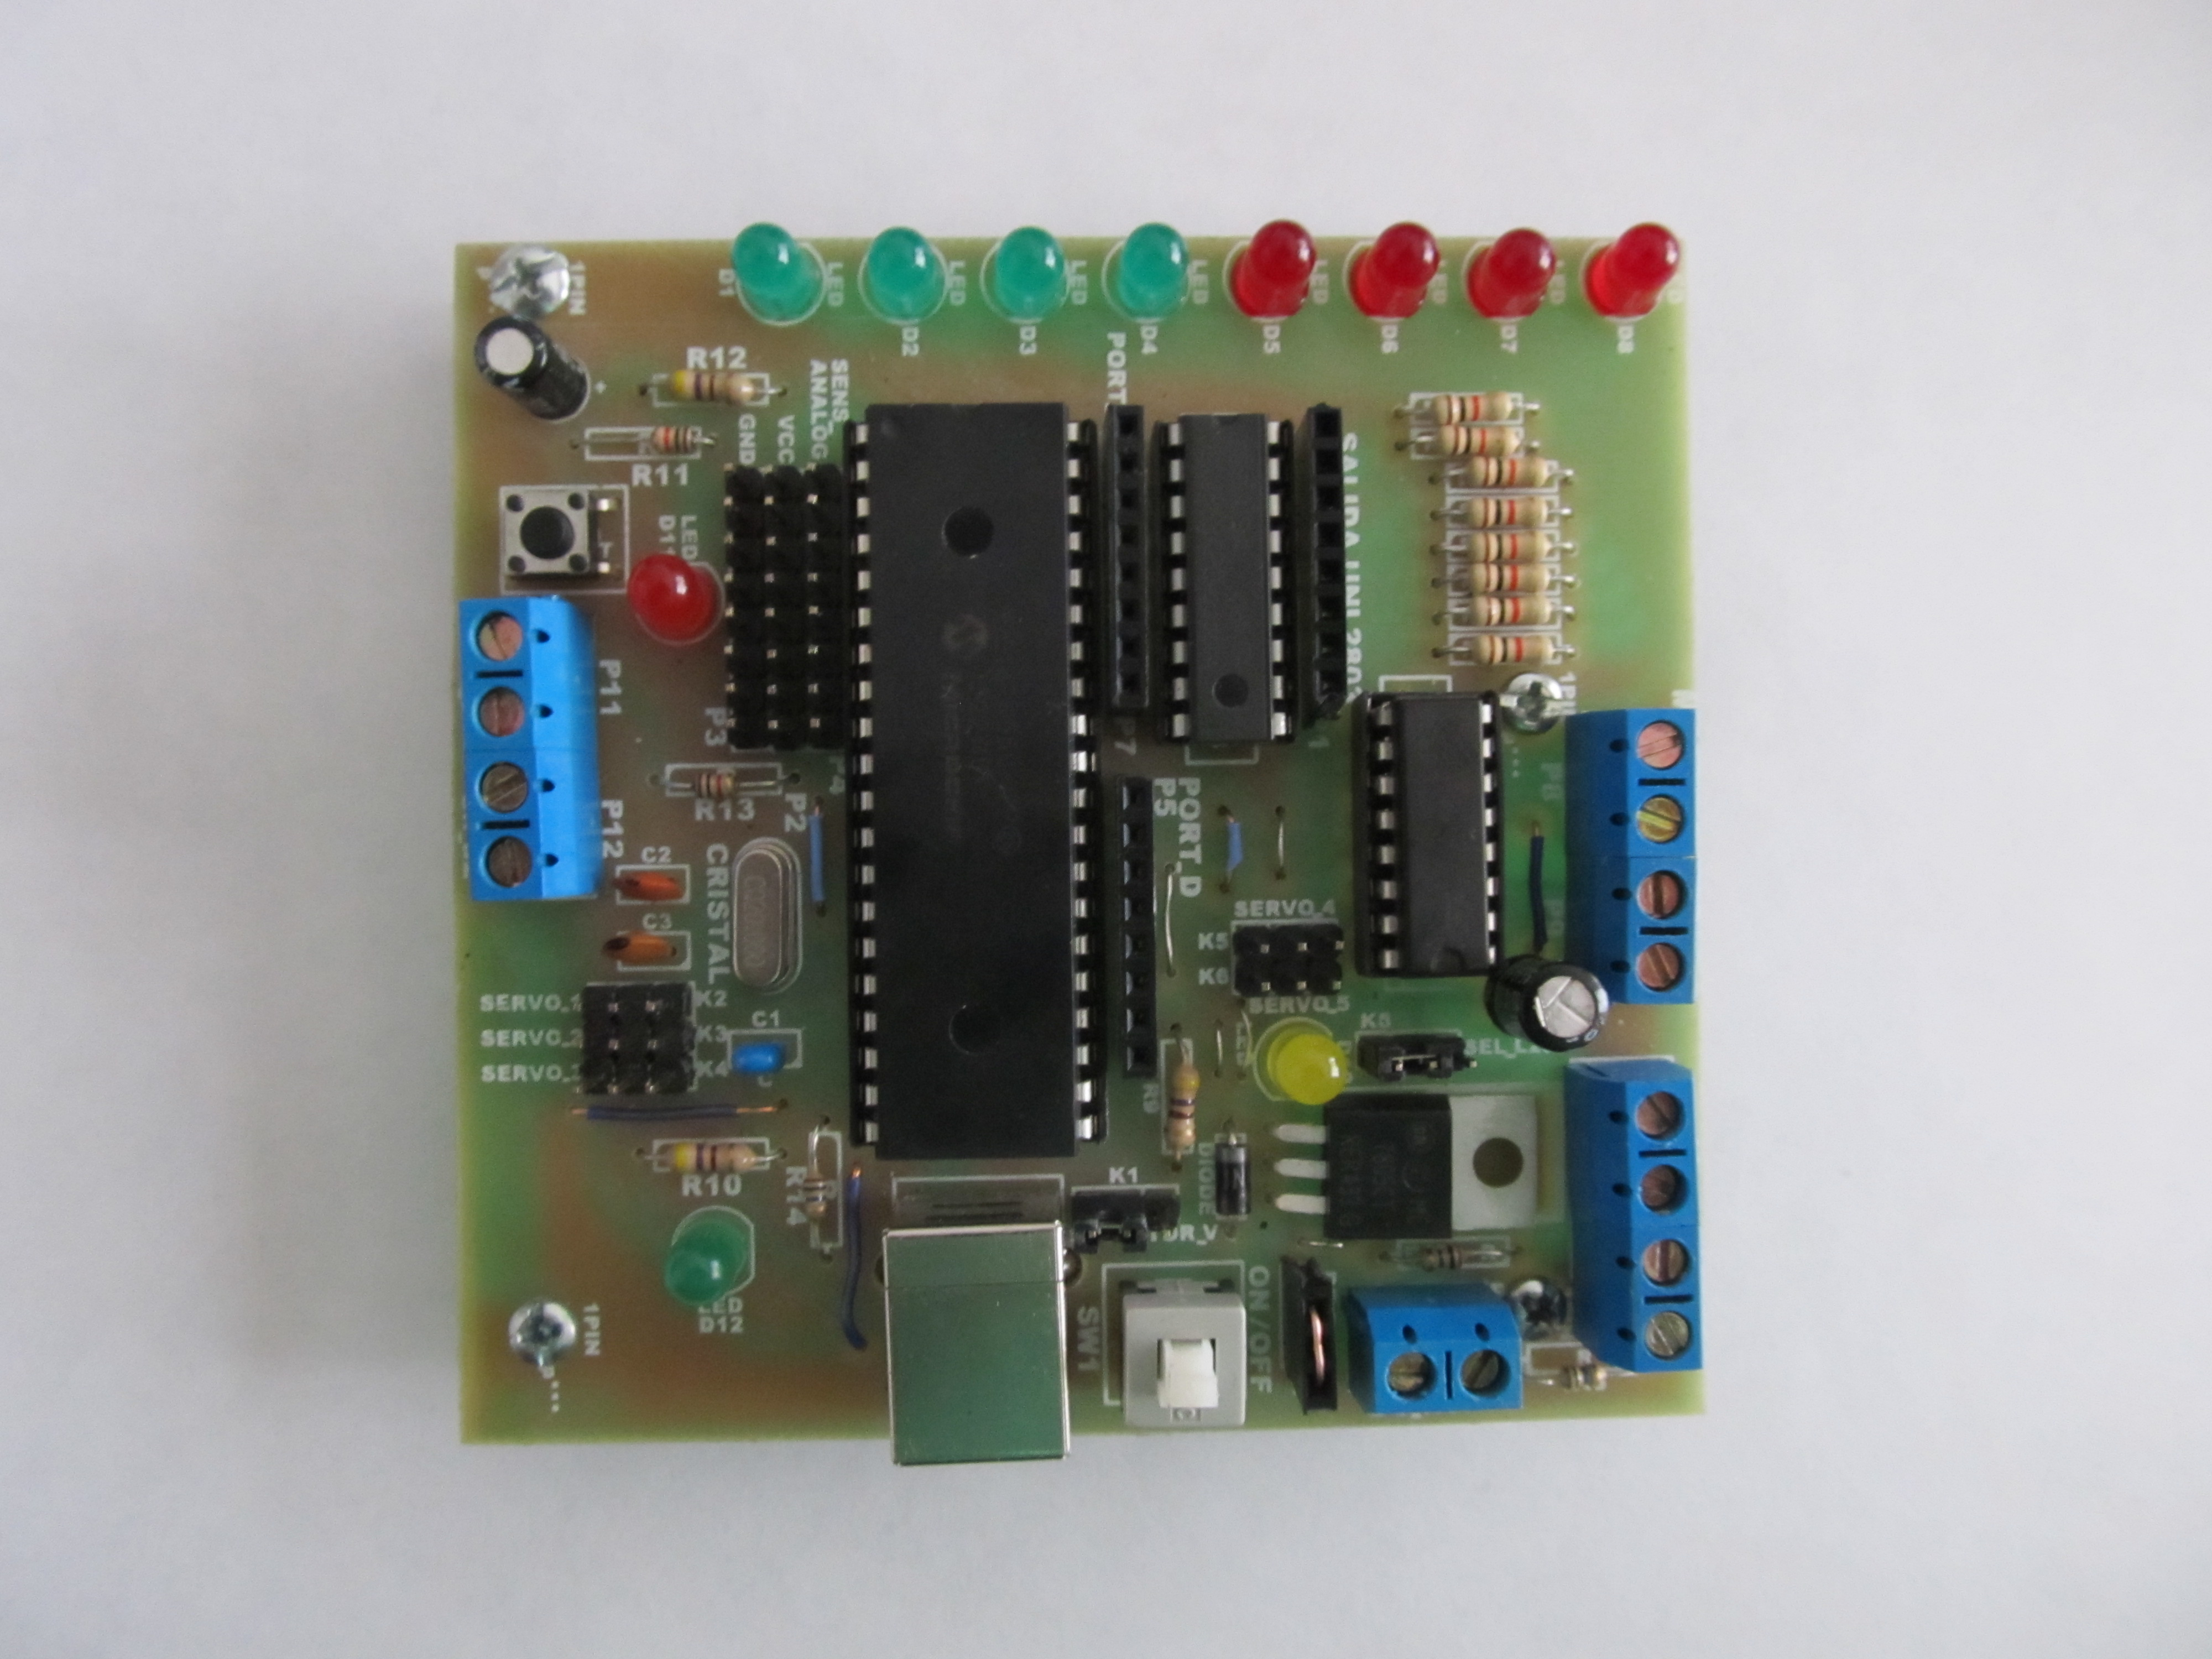
\includegraphics[width=0.5\columnwidth,height=0.5\columnwidth,keepaspectratio]{img/IMG_0134.JPG}
\par\end{centering}

\caption{placa para enseñanza de Róbotica ICARO}
\end{wrapfigure}%
 El desarrollo de estos juguetes-objetos implica una experiencia que
contribuye a expandir la creatividad y el pensamiento reflexivo y
científico de los alumnos, en relación a la formulación de hipótesis,
la experimentación y la elaboración de conclusiones. Al enfrentarse
a un “problema” dado, los estudiantes aprenden a experimentar, diseñar
y resolver situaciones de carácter constructivista. En el proceso
de “pensar el robot”, se generan las condiciones de apropiación del
conocimiento por parte del alumno. Se trata de otorgar a los alumnos
un rol activo en sus aprendizajes, colocándolos como diseñadores de
sus propios proyectos y constructores de conocimientos. A su vez,
el uso de software libre permite tener control sobre las características
del mismo, permitiendo adaptarlo a las necesidades concretas del ámbito
escolar y las realidades socio-económicas de la institución, es neutro
frente a fabricantes y todo el material usado puede ponerse a disposición
de otros docentes.

Las <<placas ICARO>> están diseñadas para poder ser fabricadas a
pequeña escala, con herramientas sencillas y con componentes de fácil
adquisición en la provincia. 

El núcleo del hardware se basa en el micro controlador PIC 18f4550
de la firma microchip™, un micro controlador barato y muy potente
con capacidad para comunicación USB y control de señales analógicas
y digitales. El software de control forma parte del Programa Nacional
Conectar Igualdad y está pre instalado en el sistema operativo Huayra
GNU/Linux de las netbooks entregadas por el Estado en el marco de
dicho programa.


\section*{Objetivos generales}
\begin{itemize}
\item Capacitar a los docentes y alumnos de los colegios técnicos de la
provincia de Córdoba en el diseño y fabricación del hardware ICARO
para robótica y automatización industrial, posibilitando la apropiación
de la tecnología para proyectos pedagógicos.
\item Introducir a los docentes en el uso y desarrollo de proyectos educativos
basados en software y hardware libre.
\item Promover el uso del sistema operativo Huayra GNU/Linux.
\item Generar unidades de producción local de hardware para que los alumnos
puedan disponer de placas electrónicas de alta potencia de procesamiento
y bajo costo para sus proyectos escolares.
\end{itemize}

\section*{Objetivos específicos}
\begin{itemize}
\item Aprender programación de lenguaje C para micro controladores PIC con
el compilador libre, SDCC.
\item Utilizar el lenguaje de programación PYTHON, para interactuar con
el hardware usando el puerto USB.
\item Usar herramientas de software libre para diseño de circuitos electrónicos
(KICAD).
\item Fabricar placas ICARO y aprender sobre su funcionamiento.
\item Diseñar un robot o un pequeño sistema de automatización.
\end{itemize}

\section*{Contenidos}
\begin{itemize}
\item Introducción a la Robótica Educativa.
\item Presentación de proyecto ICARO de robótica educativa con software
y hardware libre.
\item Introducción al software libre.
\item Uso del sistema operativo Huayra GNU/Linux del Programa Conectar Igualdad.
\item Nociones básicas de programación con lenguaje PYTHON.
\item Pruebas de programación de micro controladores PICs 18f4550.
\item Sensores de Contacto, sensores de Luz, sensores de ultra sonido.
\item Servos motores, motores CC, motores PAP.
\item Comunicación y control del hardware vía puerto USB.
\item Uso del software libre para diseño de circuitos electrónicos KICAD.
\item Introducción al uso de software para diseño CAD/CAM 3d con FREECAD.
\end{itemize}

\section*{Plan y estrategias de trabajo}

El curso de Robótica se desarrollará durante cuatro semanas en horario
curricular o extracurricular (un día a la semana, tres horas reloj).
Las actividades se llevarán a cabo en un salón con buena iluminación,
dotado con espacio para que los alumnos puedan trabajar con sus netbooks.
\begin{wrapfigure}{o}{0.5\columnwidth}%
\begin{centering}
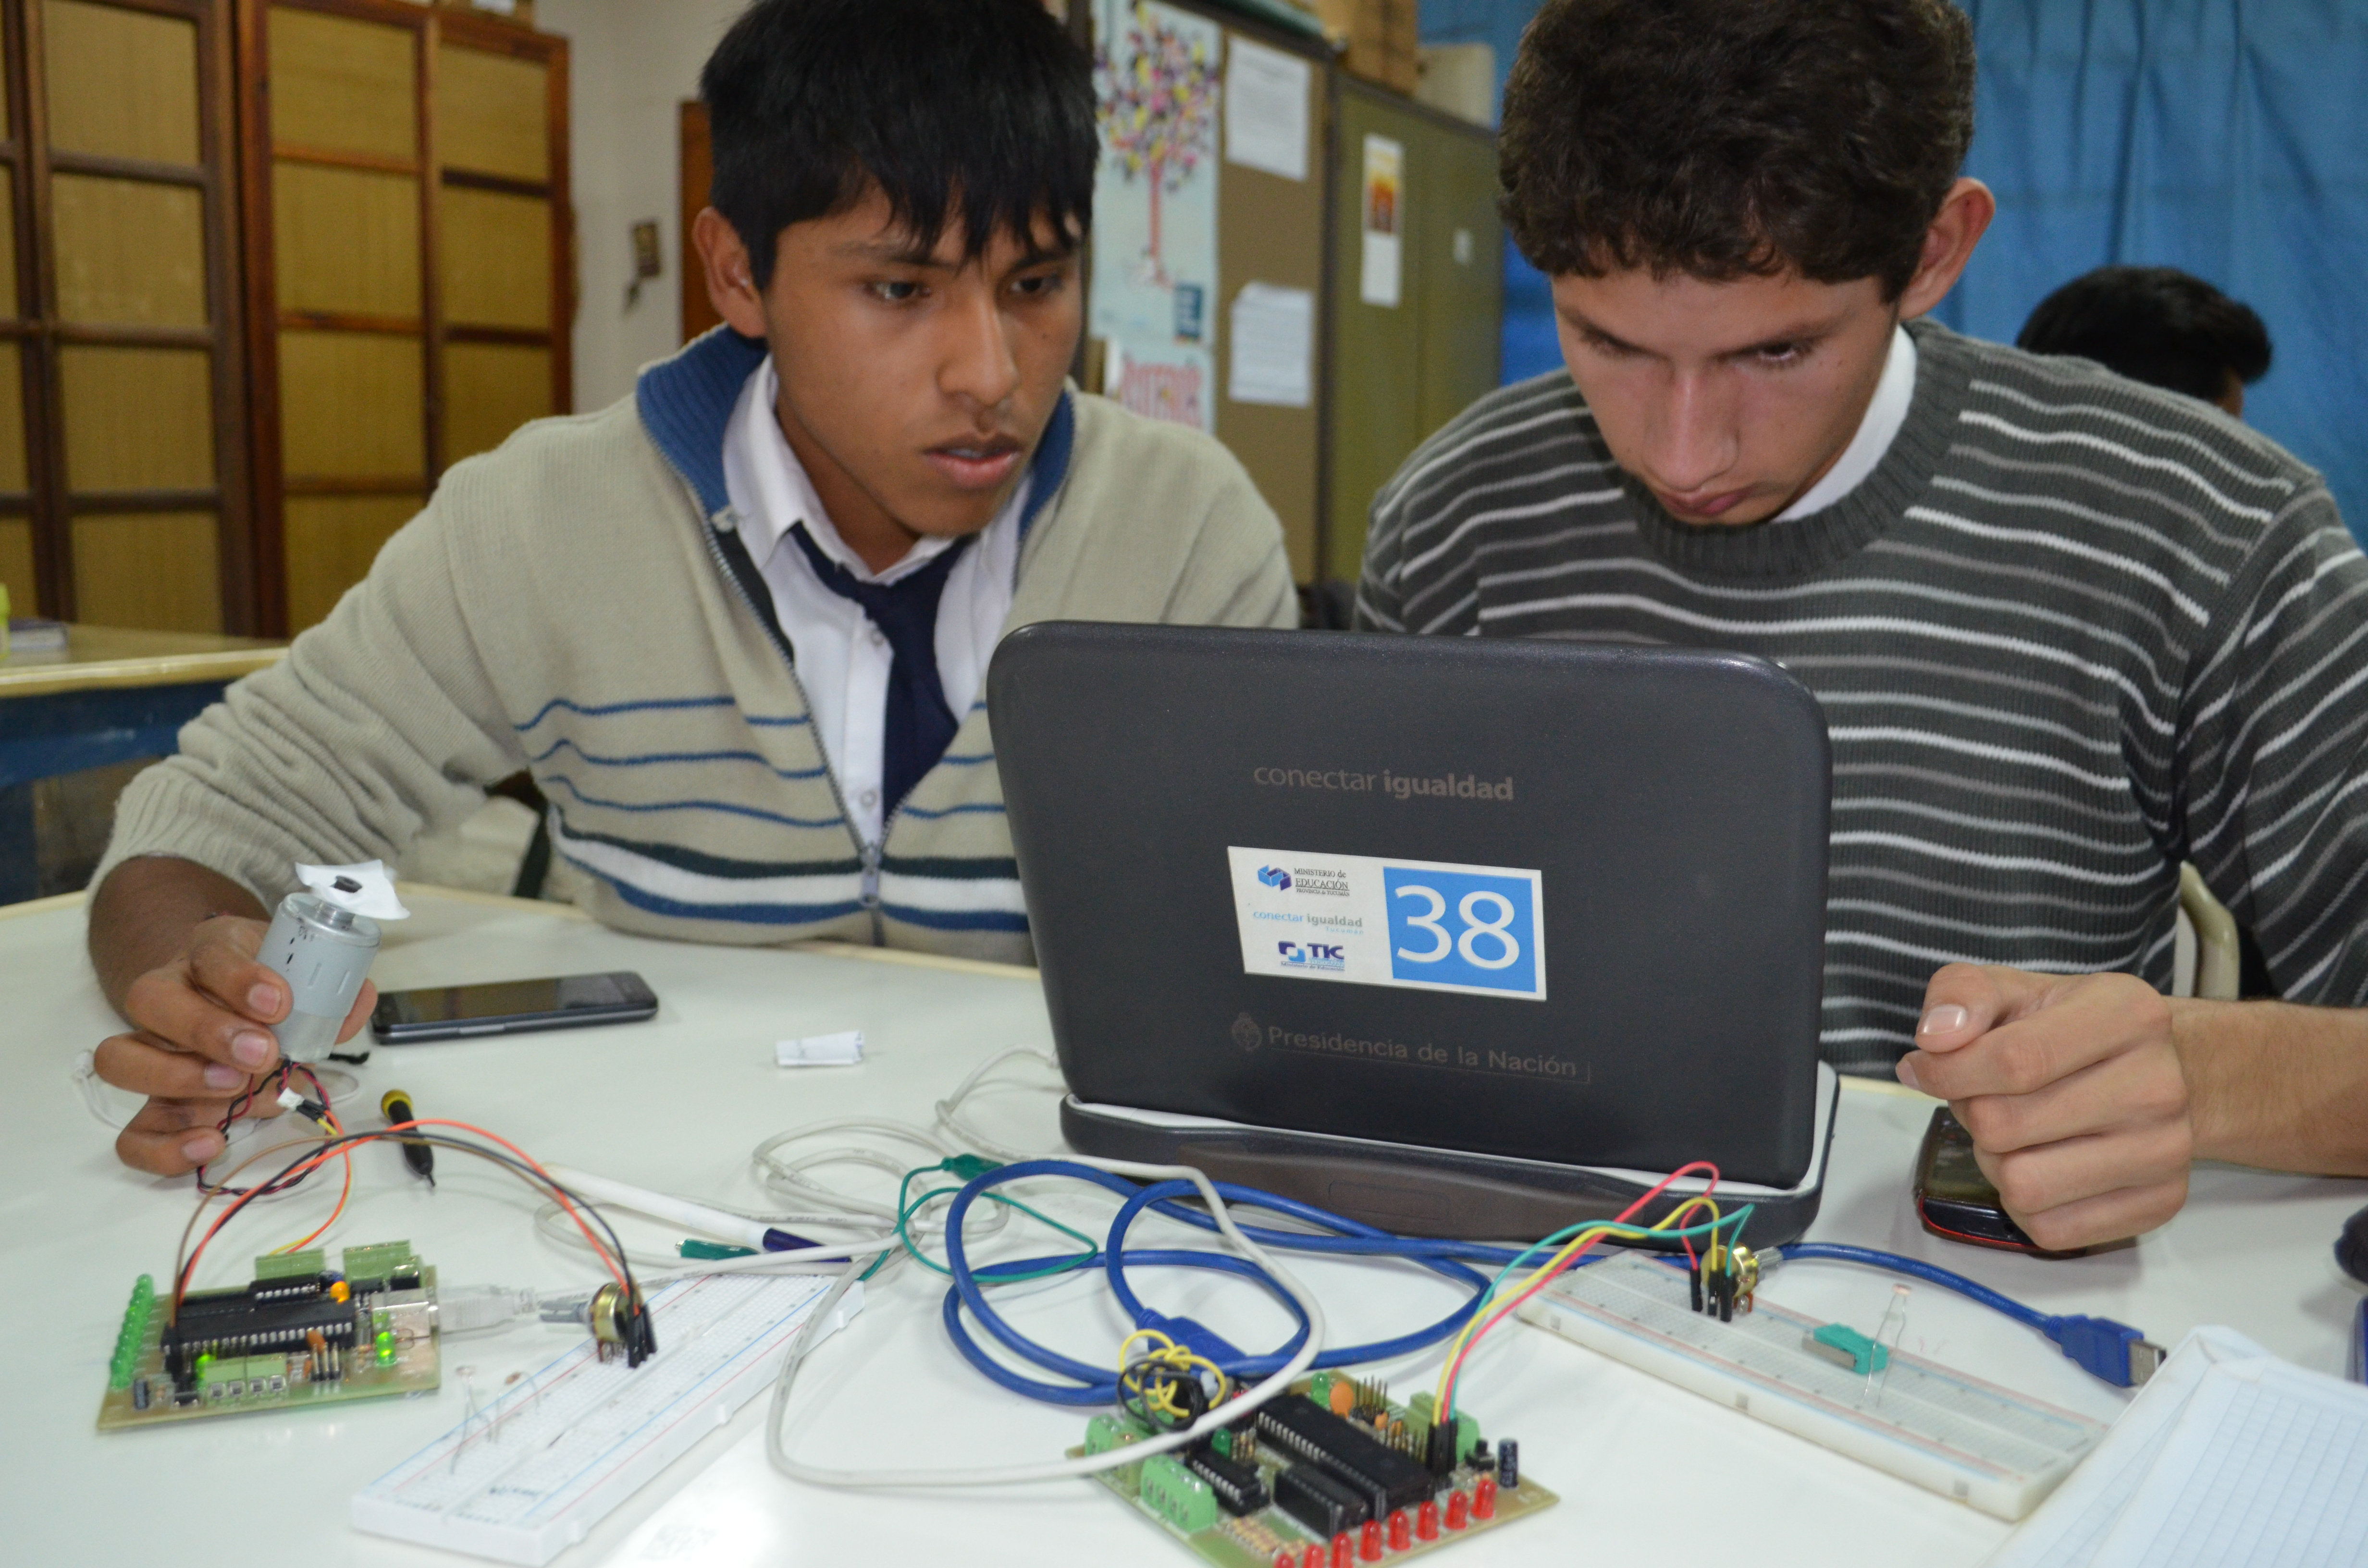
\includegraphics[width=0.5\columnwidth,height=0.5\columnwidth,keepaspectratio]{img/DSC_0334.JPG}
\par\end{centering}

\caption{Alumnos usando ICARO}
\end{wrapfigure}%
 

El cupo máximo por curso será de 25 personas. Para desarrollar las
actividades, los participantes del curso se dividirán en grupos integrados
por cinco alumnos. En el caso de que participe en el curso más de
un colegio, los grupos estarán conformados por un docente y cuatro
alumnos. Cada grupo deberá contar con al menos una netbook -con el
sistema operativo Huayra GNU/Linux instalado-, un soldador de estaño,
un alicate, un PCB ICARO y los componentes necesarios para poder fabricar
el hardware. 


\section*{Cronograma}

El Cronograma de cursado se dividirá en cuatro clases presenciales
de tres horas cada una con el siguiente formato:
\begin{itemize}
\item 1° clase. Presentación del proyecto ICARO, introducción al hardware,
electrónica y programación de la placa, nociones de algoritmos.
\item 2° clase. Fabricación del hardware.
\item 3° clase. Uso de motores CC, servo motores y motores PAP.
\item 4° clase. Prueba de sensores analógicos y digitales, control del hardware
desde la netbook. Finalización del curso.
\end{itemize}

\section*{Recursos}

Para cada curso se necesitarán los siguientes elementos, por grupo:
\begin{itemize}
\item Soldador de estaño, alicates, tester, estaño y des soldador.
\item Pcb ICARO y componentes para fabricar cada placa (componentes electrónicos).
\item Netbook del Programa Conectar Igualdad con el sistema operativo HUAYRA
GNU/Linux.
\end{itemize}
Recursos pedagógicos:
\begin{itemize}
\item Pizarrón
\item Cañón proyector
\item Espacio de trabajo con mesas para cada grupo y conexión eléctrica.\end{itemize}

\end{document}
